\chapter{Návrh}
\label{sec:de}

\section{Návrhový vzor MVC}
\label{sec:de_mvc}

Struktura nadřazeného systému je vhodná k~použití návrhového vzoru MVC, tedy \textit{model-view-controller}. \textit{Model} zde představují garáže (podřízené systémy), k~nim vázané události a logika jejich vyhodnocování. 

\textit{View} je zobrazení těchto dat, tedy především generované HTML stránky webového rozhraní. Jako další \textit{view} je možné považovat získávání dat (například ve formátu JSON) pomocí API nadřazeného systému, třeba při zasílání registračních klíčů podřízeným systémům.

\textit{Controller} je pak část aplikace, která se stará o~zpracování HTTP požadavků. Ty mohou přicházet jednak z~uživateloval prohlížeče, jednak od podřízených systémů. Na základě těchto požadavků pak \textit{controller} posílá příslušné příkazy \textit{modelu}. Struktura aplikace při použití vzoru MVC je naznačena na obrázku \ref{fig:mvc}.

\begin{figure}[h!]
    \centering
    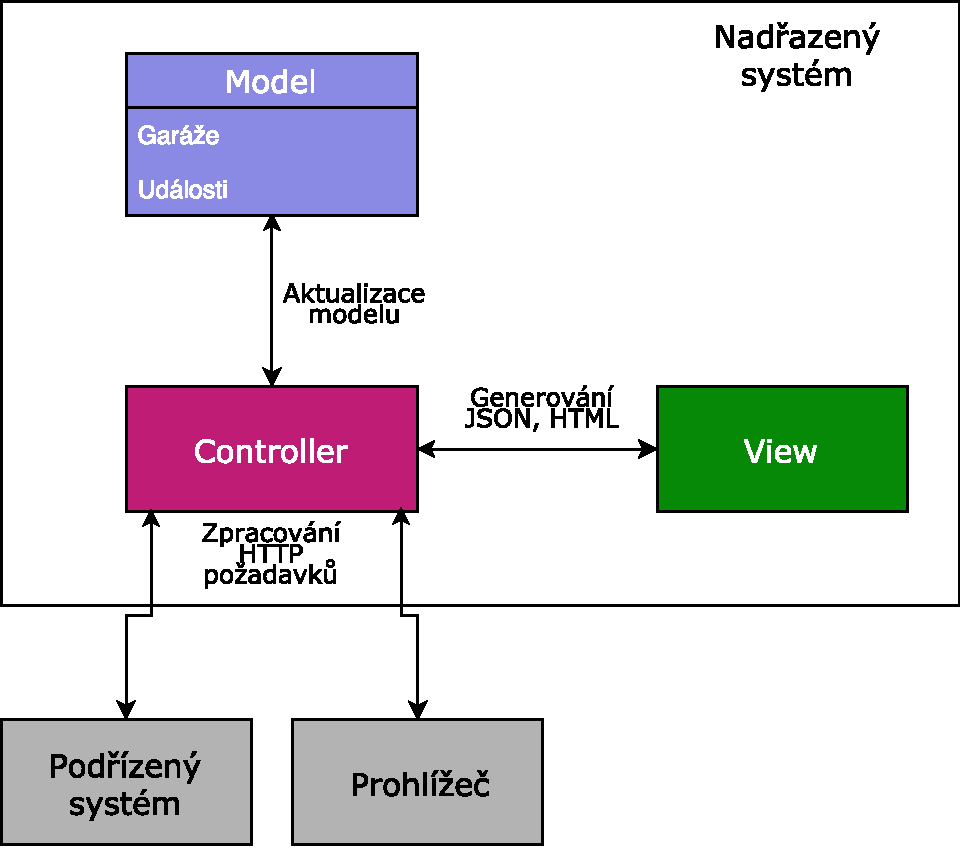
\includegraphics[width=\textwidth]{images/mvc.pdf}
    \caption[Struktura MVC aplikace]{Struktura MVC aplikcace. Uživatel i podřízený systém používají aplikaci pomocí \textit{controlleru}. Ten definuje příslušná URL a zpracovává požadavky na ně -- aktualizuje \textit{model}, případně doručí odpovídající \textit{view}}
    \label{fig:mvc}
\end{figure}

Hlavní motivací pro použití tohoto vzoru je snadná rozšiřitelnost. Pokud by například bylo potřeba aplikaci doplnit o~komunikaci s~podřízenými systémy pomocí MQTT, stačí pouze vytvořit vhodný \textit{controller}. Ten pak může využívat \textit{model} aplikace stejným způsobem jako HTTP \textit{controller}.

Tento návrhový vzor popisuje pouze nadřazený systém spravující garáže. Kromě toho je součástí aplikace ještě autentizace uživatele při přístupu do uživatelského rozhraní. Tuto funkci jsem se rozhodl pojmout jako samostatnou komponentu, popsanou v~sekci \ref{sec:de_auth}.

\section{\textit{Model}}
\label{sec:de_model}

\textit{Model} představuje jádro nadřazeného systému. Je zde implementována vnitřní reprezentace uchovávaných dat, což jsou především zaznamenané události. Každá událost má také svého původce, tedy garáž (přesněji podřízený systém v~této garáži).

Kromě toho \textit{model} implementuje \textit{business logiku} sytému, jako je například vytváření nových garáží (registraci podřízených systémů) či reakce na příchozích události.

Ostatní části aplikace (\textit{view} a \textit{controller}) používají \textit{model}, bez znalosti jeho vnitřní struktury, pomocí následujících operací:

\begin{itemize}
    \item \textbf{Vytvoření garáže} -- registrace nového podřízeného systému. V~případě vytváření pomocí API (tj. přímo podřízeným systémem) vyžaduje operace zapnutý registrační mód. Pokud je nová garáž vytvářena ve webovém rozhraní, zapnutý registrační mód není vyžadován.
    \item \textbf{Editace garáže} -- například změna označení.
    \item \textbf{Smazání garáže} -- smazáním garáže dojde k~odstranění zaznamenaných událostí a zneplatnění příslušného API klíče.
    \item \textbf{Zneplatnění API klíče} -- odepření přístupu podřízenému systému bez nutnosti smazání garáže a s~ní spojených událostí.
    \item \textbf{Zapínání registračního módu} -- v~tomto módu je možné vytvářet nové garáže na základě požadavku od podřízeného systému. Bližší informace jsou v~sekci \ref{sec:de_add_garage}. Registrační mód se po uplynutí časového limitu sám vypne.
    \item \textbf{Přístup k~uloženým datům} -- obecně operace typu získání všech garáží nebo všech událostí vázané ke konkrétní garáži.
    \item \textbf{Vytvoření události} -- základní požadavek využívaný podřízenými systémy.
\end{itemize}

Vnitřně pak model na základě těchto operací autentizuje pomocí API klíčů požadavky podřízených systému, validuje zaslaná data, spravuje databázi nadřazeného systému nebo obstarává zasílání notifikačních e-mailů.

\subsection{Garáž -- \texttt{Garage}}

Třída \texttt{Garage} reprezentuje konkrétní podřízený systém a uchovává s~ním spojená data:

\begin{itemize}
    \item \texttt{id} -- identifikace entity v~databázi.
    \item \texttt{tag} -- uživatelem zvolené označení garáže. To slouží pro snadnější orientaci ve webovém rozhraní (uživatel nemusí garáže rozlišovat podle nic neříkajícího \texttt{id}).
    \item \texttt{note} -- poznámka pro další popis garáže.
    \item \texttt{api\_key} -- klíč umožňující přístup k~API systému. Ten je také zaslán zařízení při jeho registraci. Generování a správa klíčů je blíže popsána v~sekci \ref{sec:de_apikeys}.
    \item \texttt{last\_report} -- datum a čas posledního kontrolního hlášeí.
    \item \texttt{next\_report} -- datum a čas dalšího očekávaného hlášení.
    \item \texttt{period} -- perioda kontrolních hlášení.
    \item \texttt{doors} -- stav dveří garáže (otevřeno/zavřeno).
    \item \texttt{state} -- celkový stav garáže (v~pořádku, nehlásí se atd.).
    \item Seznam událostí spojených s~touto garáží.
\end{itemize}

\subsubsection{Vytváření nových garáží}
\label{sec:de_add_garage}

Nové garáže mohou v~systému vznikat dvěma způsoby. První možnost je vytvoření nové garáže přímo v~uživatelském rozhraní. Po vytvoření se zde zobrazí vygenerovaný API klíč, který je potřeba nahrát na příslušný podřízený systém. Způsob nahrávání by závisel na příslušném hardwaru (například sériová linka). Tato možnost je určena především pro podřízené systémy, které by nepodporovaly zaslání registračního požadavku a nevyžaduje zapnutý registrační mód.

Druhá možnost je použít registrační mód. V~tom případě je nová garáž vytvořena na základě registračního požadavku podřízeného systému (pro bližší informace o~tomto požadavku viz sekci \ref{sec:de_api}). Vygenerovaný API klíč je při tom zaslán jako odpověď na požadavek, a není tedy nutné ho ručně nahrávat. Registrační mód je možné aktivovat v~uživatelském rozhraní. Pokud mód není aktivovaný, nadřazený systém odmítne všechny požadavky na registraci zaslané tímto způsobem.

\subsubsection{API klíče}
\label{sec:de_apikeys}

Podřízené systému se při zasílání událostí přes API prokazují klíčem. Ten slouží jednak k~zamezení příjmu událostí od neautorizovaných systému, jednak k~identifikaci původu události (zdrojové garáže) v~rámci nadřazeného systému. Podřízený systém tedy nemusí znát \texttt{id} garáže, ale jen \texttt{api\_key}.

%generovani klice
Vzhledem k~těmto požadavkům nelze použít jeden univerzální, ale je nutné pro každý registrovaný podřízený systém vygenerovat unikátní klíč. Ten je pak spolu s~dalšími záznamy o~garáži uložen v~databázi systému. K~vytváření klíčů jsem se rozhodl použít systém UUID, umožňující generování náhodných klíčů délky 128 bitů, které jsou (pro praktické účely) unikátní \cite{rfc4122}.

Klíče je možné v~uživatelském rozhraní zneplatnit, a tím odepřít přístup zvolenému podřízenému systému. Tuto operaci lze provést dvěma způsoby. V~prvním případě lze smazat z~databáze celý záznam příslušné garáže. Tím dojde k~zneplatnění jejího klíče, ale také k~odstranění zaznamenaných událostí.

Pokud si uživatel přeje data o~událostech uchovat, může pouze vygenerovat nový API klíč. Přepsáním klíče se opět zneplatní přístup podřízeného systému (který má stále starý klíč), ale uchovají se zaznamenaná data. 

Nově vygenerovaný klíč pak uživatel může nahrát na jiný podřízený systém, a tím například nahradit odcizené monitorovací zařízení. V~tomto případě nelze pro nahrání klíče použít registrační mód nadřazeného systému. Ten totiž vždy počítá s~vytvořením nové garáže.

Vygenerované klíče jsou v~databázi uloženy v~čitelné podobě. Klíče by bylo možné před uložením \textit{hashovat}, čímž by při úniku databáze nedošlo k~jejich prozrazení. V~tom případě by byl klíč v~čitelné podobě v~uživatelském rozhraní zobrazen pouze jednou, při vytvoření nové garáže. Dále už by byl uchováván jeho \textit{hash}.

Pro ukládání klíčů v~čitelné podobě jsem se rozhodl především z~důvodů snadného ladění při implementaci nadřazeného a podřízených systémů. Funkci \textit{hashování} klíčů by v~případě potřeby neměl být problém doplnit.

\subsection{Událost -- \texttt{Event}}
\label{sec:de_event}

Třída \texttt{Event} představuje událost zaznamenanou podřízeným systémem. Jak bylo zmíněno v~sekci \ref{sec:de_mvc}, jsou tyto události vázány ke konkrétním garážím, kdy každá událost má jednoznačně určeného původce, a každá garáž libovolné množství událostí.

Nadřazený systém rozlišuje dva základní druhy událostí. Kontrolní (plánované) události slouží ke kontrole funkčnosti podřízených systémů. Tyto události jsou odesílány v~pravidelném intervalu, určeném nadřazeným systémem. Ten v~odpovědi na požadavek s~kontrolní událostí zašle očekávaný čas (počet minut) do dalšího hlášení.

Kromě kontrolních hlášení mohou podřízené systémy vytvářet mimořádné události. Mimořádná událost nastane při překročení mezních hodnot některého z~čidel (tedy detekce kouře, pohybu či otevření/zavření dveří).

Třída \texttt{Event} obsahuje tyto údaje:

\begin{itemize}
    \item \texttt{id} -- identifikace entity v~databázi.
    \item \texttt{timestamp} -- časové razítko.
    \item \texttt{type} -- typ zaznamenané události. Nadřazený systém rozeznává následující typy:
    \begin{itemize}
        \item \texttt{report} -- kontrolní hlášení.
        \item \texttt{door\_open} -- otevření dveří.
        \item \texttt{door\_close} -- zavření dveří.
        \item \texttt{movement} -- detekce pohybu.
        \item \texttt{smoke} -- detekce kouře.
    \end{itemize}
    \item Garáž, která je původcem události.
\end{itemize}

\subsubsection{Vyhodnocení události}

\begin{figure}[h!]
    \centering
    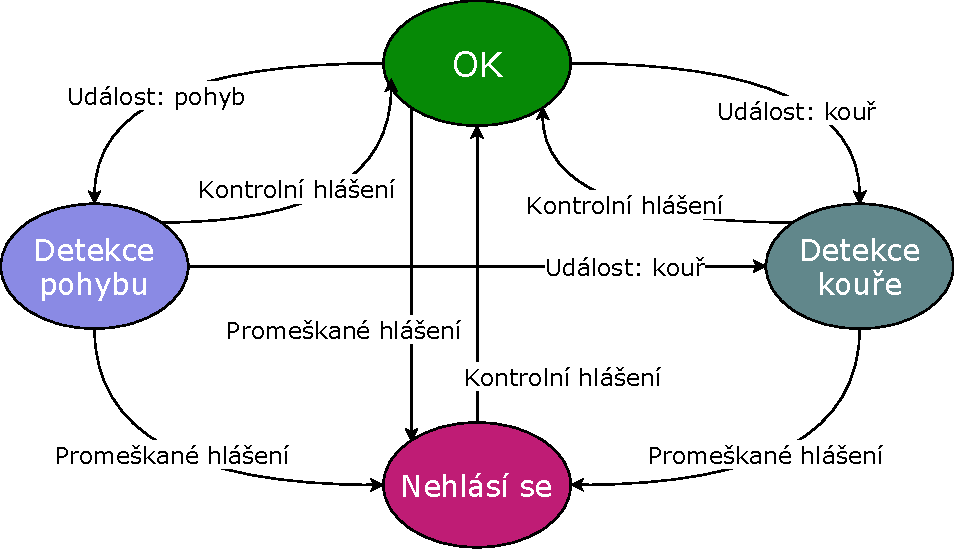
\includegraphics[width=\textwidth]{images/garage_state.pdf}
    \caption[Diagram vyhodnocování stavu garáže]{Diagram vyhodnocování stavu garáže. Nadřazený systém reaguje na příchozí události odpovídající změnou stavu garáže. Změna stavu může být také vyvolána při pravidelné kontrole propásnutých hlášení (přechod do stavu \uv{Nehlásí se})}
    \label{fig:garage_state}
\end{figure}

Příchozí události a stav garáže jsou nadřazeným systémem vyhodnocovány na základě diagramu na obrázku \ref{fig:garage_state}. Změna stavu nastává buď v~reakci na příchozí událost (například detekci kouře) nebo při pravidelné kontrole zaslaných hlášení. 

Pokud při této kontrole nadřazený systém zjistí, že neobdržel očekávané kontrolní hlášení, změní stav garáže na \textcolor{magenta}{\uv{Nehlásí se}}. Tato změna nastane vždy, bez ohledu na předchozí stav. Ze stavu \textcolor{magenta}{\uv{Nehlásí se}} se lze dostat pouze zasláním kontrolního hlášení.

Kontrolní hlášení funguje jako potvrzení, že jakákoliv nenadálá situace v~garáži byla vyřešena. Pokud například podřízený systém detekuje kouř, odešle příslušnou událost a pozdrží další kontrolní hlášení až do doby, kdy bude zdroj kouře odstraněn. Poté může zasláním kontrolního hlášení změnit stav garáže zpět na \textcolor{green}{\uv{OK}}.

Kromě událostí měnících stav garáže nadřazený systém ještě rozeznává události otevření a zavření dveří garáže. Tyto události nemění stav garáže, pouze aktualizují stav dveří. Nejsou tedy součástí tohoto vyhodnocování.

\subsubsection{Zasílání upozornění}

Na základě příchozích událostí odesílá nadřazený systém notifikační e-maily na adresu zvolenou uživatelem. E-mail s~příslušnou událostí je odeslán vždy při změně stavu garáže (mimo změny do stavu \uv{OK}). Tím je zamezeno zbytečnému zasílání duplicitních e-mailů.

%tady pak asi bude i jak to bude celkove s tema mailama

%taky popsat jaky sou moznosti autorizace na tim gmailu (proste smtp meno heslo a pak ty oauth veci) a ze nic z toho neni pro nas uplne idealni

%vidim to bud teda ze tam bude proste smtp klient a holt meno (pak ta emailova schranka muze bejt vicemene jakakoliv, to je taky trochu vyhoda -- tj si uzivatel zalozi stranku treba na seznamu, vyplni meno a heslo a ma to hotovy) a heslo a nebo pouzit nakou sluzbu na posilani mailu. Ten google ma tu oauth autorizaci hrozne slozitou, by asi bylo lepsi neco jako https://github.com/sendgrid/sendgrid-python (https://sendgrid.com/), tam staci proste api klic 

\section{\textit{View}}

Hlavním \textit{view} nadřazeného systému je webové uživatelské rozhraní. Zde se zobrazuje celkový stav systému, jednotlivých garáží, a zachycené události. Také jsou ze přístupné ovládací prvky pro správu systému. Návrhem tohoto rozhraní se zabývá následující sekce \ref{sec:de_web}.

Další \textit{view} aplikace představují odpovědi (například vygenerované API klíče) nadřazeného systému podřízeným systému při zpracování jejich požadavků. Tento \textit{view} je popsán společně s~API systému v~sekci \ref{sec:de_api}.

\subsection{Webové rozhraní}
\label{sec:de_web}

Webové rozhraní představuje prostředí umožňující uživatel správu celého nadřazeného systému. Rozhraní tvoří hlavní stránka, stránky jednotlivých garáží a stránky uživatelského nastavení (změna hesla a nastavení notifikací).

Případy užití rozhraní se dají shrnout do tří kategorií, popsaných na obrázku \ref{fig:use_case_top}.

\begin{figure}[h!]
    \centering
    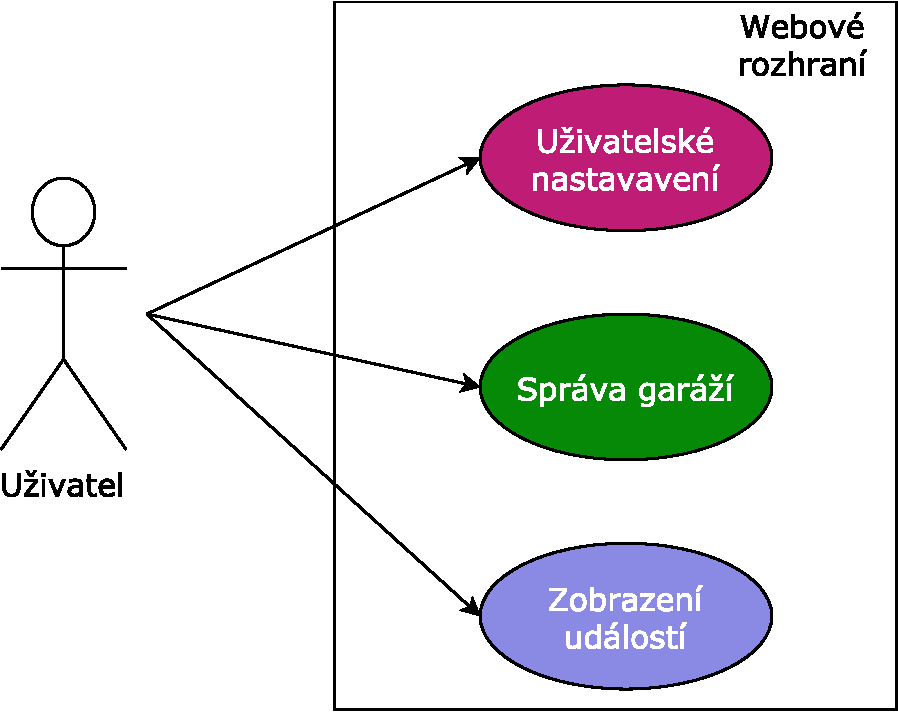
\includegraphics[width=0.9\textwidth]{images/use_case_top.pdf}
    \caption[Vrchní úroveň případů užití webového rozhraní]{Vrchní úroveň případů užití webového rozhraní. Uživatel do aplikace přistupuje buď za účelem změny uživatelského nastavení, správy jednotlivý podřízených systémů, případně kvůli kontrole zaznamenaných událostí}
    \label{fig:use_case_top}
\end{figure}

\subsubsection{Správa garáží}

Správu garáží tvoří případy užití popsané na obrázku \ref{fig:use_case_garage}. Operace vytvoření garáže a zapnutí registračního módu nejsou vázané k~žádné konkrétní garáži, a jsou tedy k~dispozici na hlavní stránce webového rozhraní ihned po přihlášení. 

Na hlavní stránce je také zobrazen seznam všech sledovaných garáží včetně jejich stavu, posledního hlášení, dalšího plánovaného hlášení a odkazu na stránku garáže, která obsahuje zbylé možnosti, vázané ke konkrétní garáži.

\begin{figure}[h!]
    \centering
    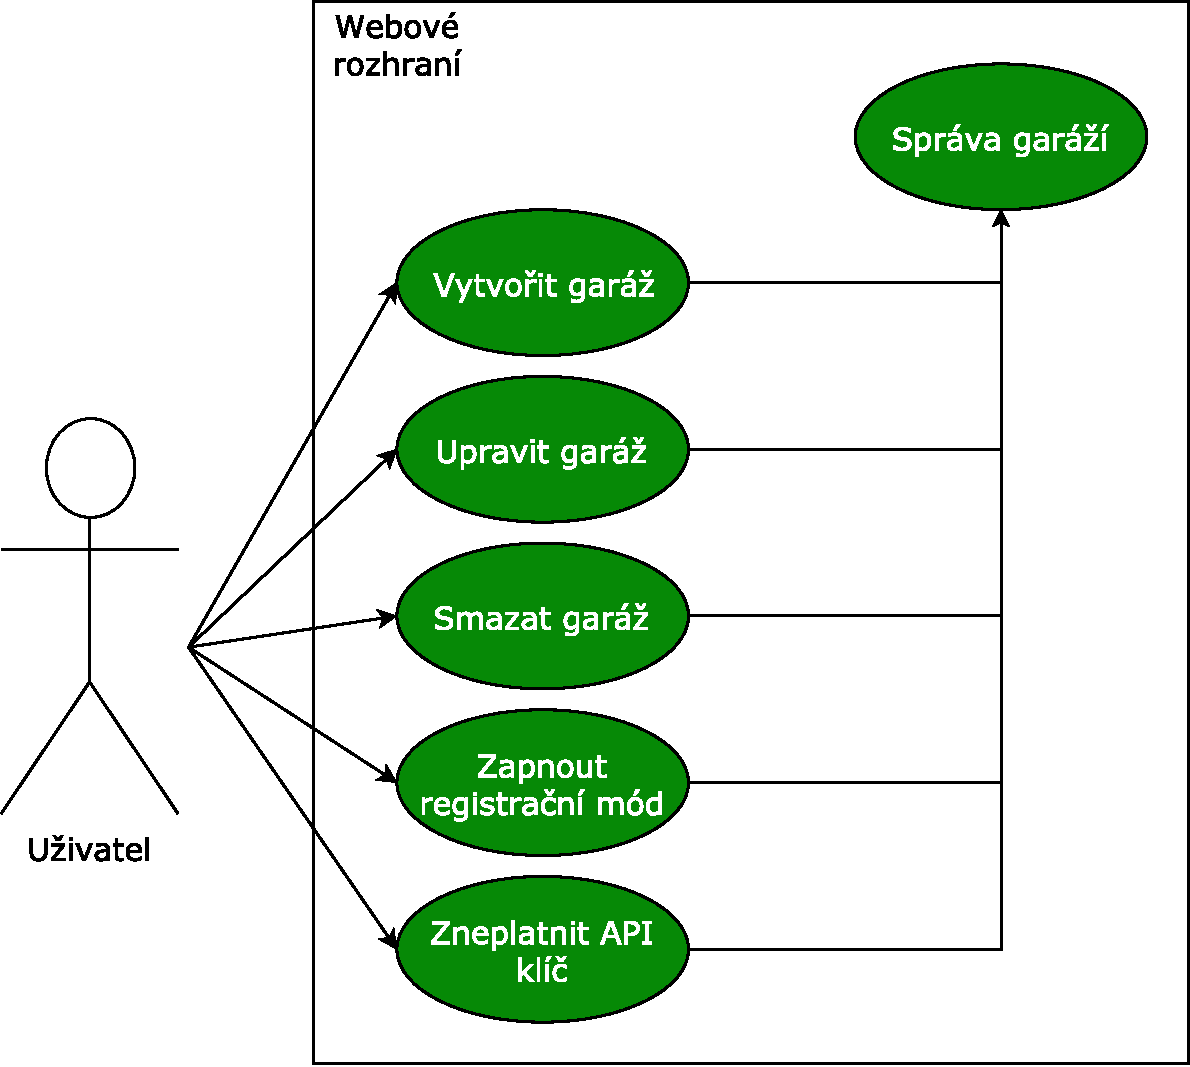
\includegraphics[width=\textwidth]{images/use_case_garage.pdf}
    \caption[Případy užití správy garáží]{Případy užití správy garáží. Zde uživatel zobrazuje stav garáží a jednotlivé garáže spravuje pomocí uvedených operací}
    \label{fig:use_case_garage}
\end{figure}

\subsubsection{Zobrazení událostí}

Případy užití z~kategorie zobrazení událostí popisuje obrázek \ref{fig:use_case_events}. Na stránce garáže může uživatel zobrazit s~ní spojené události. Seznam událostí pak může filtrovat podle typu (viz sekci \ref{sec:de_event}).

\begin{figure}[h!]
    \centering
    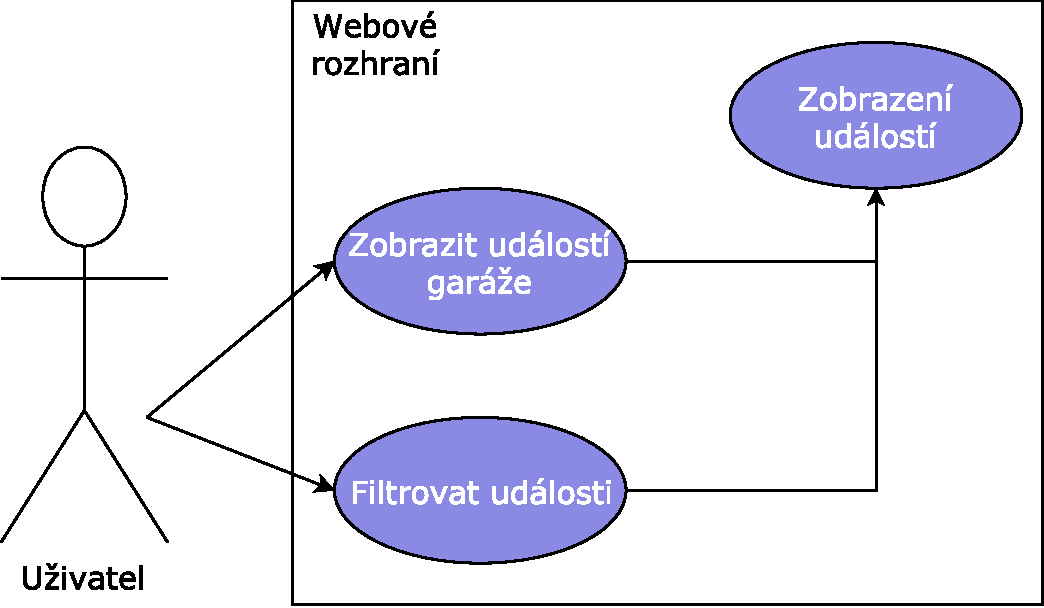
\includegraphics[width=\textwidth]{images/use_case_events.pdf}
    \caption[Případy užití zobrazení událostí]{Případy užití zobrazení událostí. Uživatel zobrazuje události spojené s~konkrétní garáží. Zobrazené událostí filtruje podle jejich typu}
    \label{fig:use_case_events}
\end{figure}

\subsubsection{Uživatelské nastavení}
\label{sec:de_user_settings}

%tady este neco bude ofc

Uživatelské nastavení není uloženo přímo v~databázi, ale zvlášť v~konfiguračním souboru \texttt{user\_settings.ini}. Díky tomu je snazší toto nastavení v~případě potřeby změnit i bez nutnosti otvírat webové rozhraní.

\begin{figure}[h!]
    \centering
    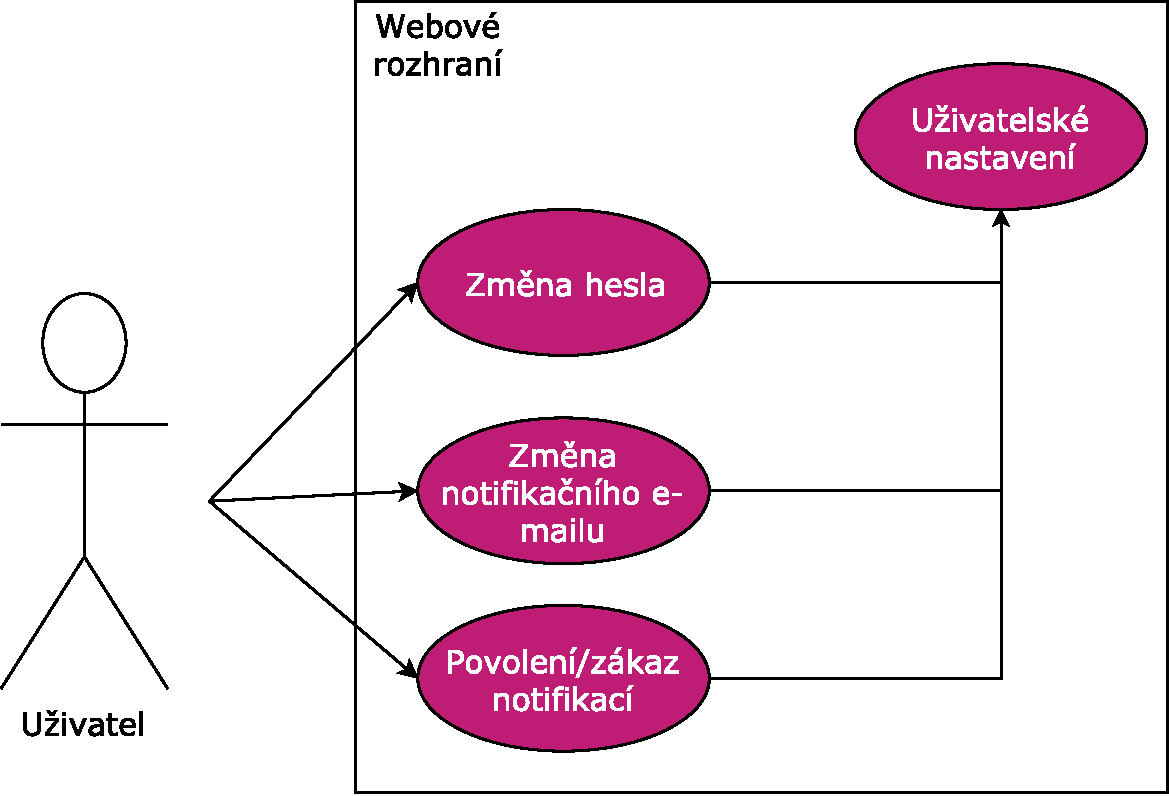
\includegraphics[width=\textwidth]{images/use_case_user.pdf}
    \caption[Případy užití uživatelského nastavení]{Případy užití uživatelského nastavení. Uživatel ve webovém rozhraní provádí změnu hesla, změnu notifikačního e-mailu, případně zákaz/povolení notifikací}
    \label{fig:use_case_user}
\end{figure}


\section{\textit{Controller}}

\textit{Controller} slouží ke zpracování požadavků uživatele a podřízených systémů. Jelikož jde o~HTTP požadavky, definuje \textit{controller} URL, přiřazuje k~nim akce, které se mají provést (kontrola přihlášení, přesměrování atd.) a vrací příslušné odpovědi (například vygenerované stránky).

\textit{Controller} aplikace se dá rozdělit na dvě části. První část zpracovává požadavky zaslané uživatelem z~webového rozhraní. Propojuje tedy případy užití popsané v~sekci \ref{sec:de_web} s~operacemi na modelu ze sekce \ref{sec:de_model}. URL definovaná v~této části jsou využívána pouze uvnitř aplikace, a nejsou součástí API nadřazeného systému.

Druhá část zpracovává požadavky podřízených systémů. Zde definovaná URL tvouří API nadřazeného systému, pomocí kterého se mohou podřízené systémy registrovat a nahrávat nové události. Popisem API, včetně formátu požadavků a návratových hodnot, se zabývá sekce \ref{sec:de_api}.

\subsection{API}
\label{sec:de_api}

%https://docs.microsoft.com/en-us/azure/architecture/best-practices/api-design

API nadřazeného systému slouží ke komunikaci s~podřízenými systémy. S~jeho pomocí se podřízený systém může registrovat a začít nadřazenému systému posílat zaznamenané události.

Odpovědi nadřazeného systému na příchozí požadavky jsou ve formátu JSON. Každá odpověď obsahuje návratový kód a případně další data, která je nutné zaslat podřízenému systému.

\subsubsection{Registrační požadavek}

Registrační požadavek slouží k~zaregistrování nového podřízeného systému a vytvoření záznamu s~ním spojené garáže. Hlavním účelem tohoto požadavku je snadná distribuce API klíče na podřízené systémy -- klíč není nutné nahrávat ručně, ale je odeslán v~odpovědi na tento požadavek (pro bližší informace o~klíčích viz sekci \ref{sec:de_apikeys}).

Kvůli bezpečnosti je tento požadavek povolen pouze pokud je v~uživatelském rozhraní zapnutný registrační mód. Pokud je mód vypnutý, odpovídá nadřazený systém na všechny registrační požadavky chybovým kódem \textit{403 -- Forbidden}. Tím je částečně zabráněno registraci nežádoucích podřízených systémů.

Registrační požadavek má následující formát (zaslání registračního požadavku v~jazycke Python je popsáno v~ukázce \ref{lst:api_reg}):

\begin{itemize}
    \item URL -- \texttt{/api/garages}.
    \item HTTP metoda -- POST.
    \item Návratová hodnota -- JSON:
    \begin{itemize}
        \item \texttt{status} -- návratový kód (201 při vytvoření garáže, 403 při vypnutém reg. módu).
        \item \texttt{api\_key} -- unikátní klíč k~API nadřazeného systému (pouze v~případě úspěchu, tedy vytvoření garáže).
    \end{itemize}
\end{itemize}

\begin{listing}[htbp]
\caption{\label{lst:api_reg} Zaslání registračního požadavku nadřazenému systému provozovaném na adrese \texttt{raspberrypi.local}}
\begin{minted}[bgcolor=codebg]{python}
import requests
# server nadrazeneho systemu je pristupny
# na adrese raspberrypi.local
url = 'https://raspberrypi.local/api/garages'

# pozadavek 'post', bez overeni
# self-signed certifikatu
r = requests.post(url, verify=False)

if r.status == 201:
    api_key = r.json()['api_key']
\end{minted}
\end{listing}

\subsubsection{Kontrolní hlášení}

Kontrolní hlášení slouží k~ověření činnosti podřízeného systému. Jeho zasláním podřízený systém také potvrzuje, že stav sledované garáže je v~pořádku. 

Požadavek zasílající kontrolní hlášení má tento formát:

\begin{itemize}
    \item URL -- \texttt{/api/report\_event}.
    \item HTTP metoda -- POST.
    \item Hlavička požadavku:
    \begin{itemize}
        \item \texttt{api\_key} -- unikátní klíč k~API nadřazeného systému.
    \end{itemize}
    \item Návratová hodnota -- JSON:
    \begin{itemize}
        \item \texttt{status} -- návratový kód (201 při vytvoření hlášení, 403 při neplatném klíči).
        \item \texttt{period} -- počet minut do dalšího očekávaného hlášení.
    \end{itemize}
\end{itemize}

\begin{listing}[htbp]
\caption{\label{lst:api_report} Zaslání kontrolního hlášení nadřazenému systému provozovaném na adrese \texttt{raspberrypi.local}}
\begin{minted}[bgcolor=codebg]{python}
import requests
# server nadrazeneho systemu je pristupny
# na adrese raspberrypi.local
url = 'https://raspberrypi.local/api/report_event'

# api klic (ziskany napriklad reg. pozadavkem)
# je zasilan v~hlavicce pozadavku
headers = {'api_key' : api_key}

# pozadavek 'post', bez overeni
# self-signed certifikatu
r = requests.post(url, headers=headers, verify=False)

if r.status == 201:
    #odpoved -- cas do dalsiho hlaseni
    period = r.json()['period']

\end{minted}
\end{listing}

\subsubsection{Ostatní události}

Vytváření dalších událostí je stejné jako vytváření kontrolního hlášení. Liší se pouze použité URL. Odpovědi na tyto požadavky neobsahují žádná data od nadřazeného systému, pouze návratový kód informující o~úspěchu či chybě:

\begin{itemize}
    \item URL -- podle typu události:
    \begin{itemize}
        \item \texttt{/api/door\_open\_event}
        \item \texttt{/api/door\_close\_event}
        \item \texttt{/api/movement\_event}
        \item \texttt{/api/smoke\_event}
    \end{itemize}
    \item HTTP metoda -- POST.
    \item Hlavička požadavku:
    \begin{itemize}
        \item \texttt{api\_key} -- unikátní klíč k~API nadřazeného systému.
    \end{itemize}
    \item Návratová hodnota -- JSON:
    \begin{itemize}
        \item \texttt{status} -- návratový kód (201 při vytvoření události, 403 při neplatném klíči).
    \end{itemize}
\end{itemize}

\begin{listing}[htbp]
\caption{\label{lst:api_report} Zaslání události detekce kouře nadřazenému systému provozovaném na adrese \texttt{raspberrypi.local}}
\begin{minted}[bgcolor=codebg]{python}
import requests

# stejne jako pri zasilani kontrolniho hlaseni
# lisi se pouze url
url = 'https://raspberrypi.local/api/smoke_event'
headers = {'api_key' : api_key}

r = requests.post(url, headers=headers, verify=False)

if r.status == 201:
    #odpoved neobsahuje zadna data
    ...

\end{minted}
\end{listing}

\section{Autentizace uživatele}
\label{sec:de_auth}

Do webového rozhraní aplikace je povolen pouze autorizovaný přístup, a je tedy nutné nějakým způsobem ověřit identitu uživatele. Jelikož aplikace nepočítá s~odlišnými stupni přístupu (a tedy každý uživatel s~přístupem do rozhraní má přístup ke všem jeho částem), rozhodl jsem se, že nebudu vytvářet infrastrukturu uživatelských účtů, protože by měla pouze omezené využití.

Přístup do rozhraní tedy nevyžaduje vytvoření účtu a zadávání uživatelského jména, ale pouze heslo. \textit{Hash} tohoto hesla (doplněného solí), vytvořený pomocí algoritmu Bcrypt, je uložen v~souboru s~uživatelským nastavením aplikace.

\textit{Hashování} hesla je zde použito především pro případ, že by uživatel použil stejné heslo jaké používá v~jiných aplikacích či službách. V~případě prozrazení uživatelských dat (například při odcizení systému) tedy útočník nemůže z~otisku zjistit původní použité heslo, tudíž přístup k~těmto uživatelovým účtům není kompromitován.

Stejně tak někdo s~přístupem k~serveru, na kterém nadřazený systém běží, nemá automaticky přístup do webového rozhraní. Nicméně má stále přístup k~celé (nešifrované) databázi a také může heslo libovolně měnit (spočítáním nového otisku), tedy z~praktického hlediska je přístup k~serveru téměř ekvivalentní s~přístupem do webového rozhraní.

\subsection{První přihlášení}

Při prvním startu nadřazeného systému je zvoleno jednoduché implicitní heslo (\textit{password}), kterým se uživatel může přihlásit do webového rozhraní. 

Pokud nadřazený systém detekuje použití tohoto hesla, po přihášení uživatele ihned přesměruje na stránku umožňující změnu hesla a zobrazí příslušné varování.